\documentclass[tikz,border=2pt]{standalone}
\usepackage{tikz}
\begin{document}
  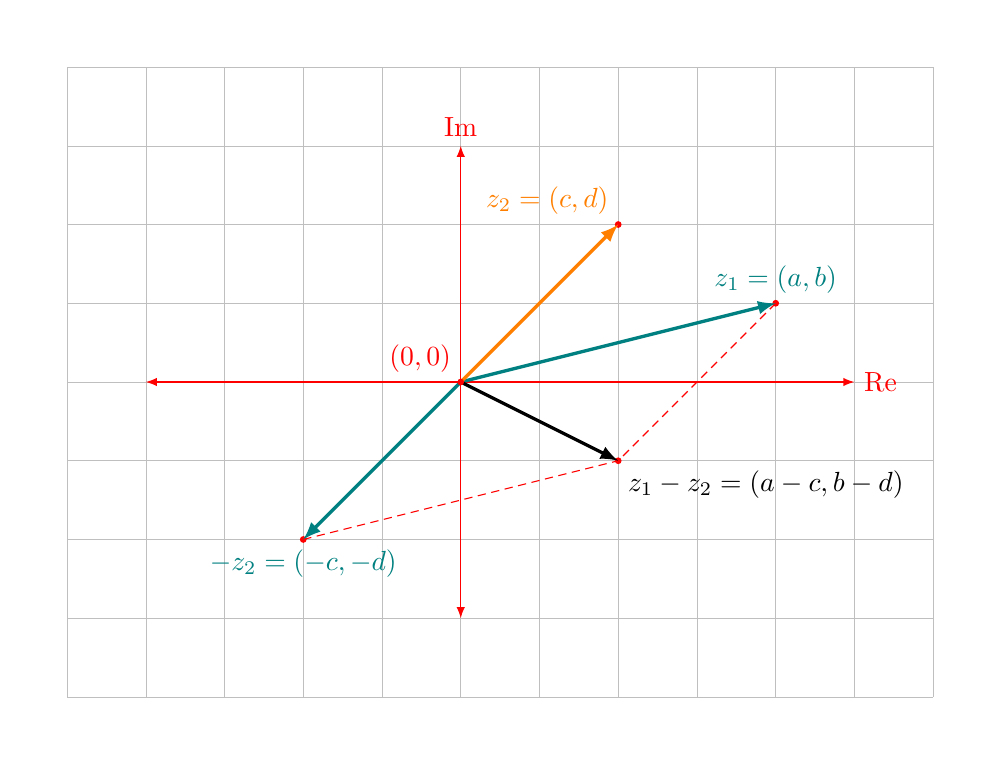
\begin{tikzpicture}
    \fill[white] (-5.5,-4.5) rectangle (6.5,4.5);
    \draw[lightgray,very thin] (-5,-4) grid (6,4);
    \draw (0,0) node[red,above left]{$(0,0)$};
    \draw[red,latex-latex] (-4,0) -- (5,0) node[right]{Re};
    \draw[red,latex-latex] (0,-3) -- (0,3) node[above]{Im};
    \draw[red,densely dashed] (4,1) -- (2,-1);
    \draw[red,densely dashed] (-2,-2) -- (2,-1);
    \filldraw[red] (2,-1) circle(1pt) node[black,below right]{$z_1-z_2=(a-c,b-d)$};
    \draw (4,1) node[teal,above]{$z_1=(a,b)$};
    \filldraw[red] (4,1) circle(1pt);
    \draw[teal,very thick,-latex] (0,0) -- (4,1);
    \draw (2,2) node[orange,above left]{$z_2=(c,d)$};
    \draw (-2,-2) node[teal,below]{$-z_2=(-c,-d)$};
    \filldraw[red] (2,2) circle(1pt);
    \filldraw[red] (-2,-2) circle(1pt);
    \draw[orange,very thick, -latex] (0,0) -- (2,2);
    \draw[teal,very thick, -latex] (0,0) -- (-2,-2);
    \draw[very thick,-latex] (0,0) -- (2,-1);
    \filldraw[red] (0,0) circle(1pt);
  \end{tikzpicture}
\end{document}
